%% Преамбула TeX-файла

% 1. Стиль и язык
\documentclass[utf8x, 14pt]{G7-32} % Стиль (по умолчанию будет 14pt)

% Остальные стандартные настройки убраны в preamble.inc.tex.
\sloppy

% Настройки стиля ГОСТ 7-32
% Для начала определяем, хотим мы или нет, чтобы рисунки и таблицы нумеровались в пределах раздела, или нам нужна сквозная нумерация.
\EqInChapter % формулы будут нумероваться в пределах раздела
\TableInChapter % таблицы будут нумероваться в пределах раздела
\PicInChapter % рисунки будут нумероваться в пределах раздела

% Добавляем гипертекстовое оглавление в PDF
\usepackage[
bookmarks=true, colorlinks=true, unicode=true,
urlcolor=black,linkcolor=black, anchorcolor=black,
citecolor=black, menucolor=black, filecolor=black,
]{hyperref}
\usepackage{pgfplots}
\usepackage{nomencl}

\usepackage{float}


\AfterHyperrefFix

\usepackage{microtype}% полезный пакет для микротипографии, увы под xelatex мало чего умеет, но под pdflatex хорошо улучшает читаемость
\usepackage{indentfirst}

% Тире могут быть невидимы в Adobe Reader
\ifInvisibleDashes
\MakeDashesBold
\fi

\usepackage{graphicx}   % Пакет для включения рисунков

% С такими полями оно работает по-умолчанию:
% \RequirePackage[left=20mm,right=10mm,top=20mm,bottom=20mm,headsep=0pt,includefoot]{geometry}
% Если вас тошнит от поля в 10мм --- увеличивайте до 20-ти, ну и про переплёт не забывайте:
\geometry{right=10mm}
\geometry{left=30mm}
\geometry{bottom=20mm}
\geometry{ignorefoot}% считать от нижней границы текста


% Пакет Tikz
\usepackage{tikz}
\usetikzlibrary{arrows,positioning,shadows}

% Произвольная нумерация списков.
\usepackage{enumerate}

% ячейки в несколько строчек
\usepackage{multirow}

% itemize внутри tabular
\usepackage{paralist,array}

%\setlength{\parskip}{1ex plus0.5ex minus0.5ex} % разрыв между абзацами
\setlength{\parskip}{1ex} % разрыв между абзацами
\usepackage{blindtext}

% Центрирование подписей к плавающим окружениям
%\usepackage[justification=centering]{caption}

\usepackage{newfloat}
\DeclareFloatingEnvironment[
placement={!ht},
name=Equation
]{eqndescNoIndent}
\edef\fixEqndesc{\noexpand\setlength{\noexpand\parindent}{\the\parindent}\noexpand\setlength{\noexpand\parskip}{\the\parskip}}
\newenvironment{eqndesc}[1][!ht]{%
    \begin{eqndescNoIndent}[#1]%
\fixEqndesc%
}
{\end{eqndescNoIndent}}

\usepackage{afterpage}

\newcommand\blankpage{
	\null
	\thispagestyle{empty}
	\newpage
}



% Настройки листингов.
\ifPDFTeX
% 8 Листинги

\usepackage{listings}

% Значения по умолчанию
\lstset{
  basicstyle= \footnotesize,
  breakatwhitespace=true,% разрыв строк только на whitespacce
  breaklines=true,       % переносить длинные строки
%   captionpos=b,          % подписи снизу -- вроде не надо
  inputencoding=koi8-r,
  numbers=left,          % нумерация слева
  numberstyle=\footnotesize,
  showspaces=false,      % показывать пробелы подчеркиваниями -- идиотизм 70-х годов
  showstringspaces=false,
  showtabs=false,        % и табы тоже
  stepnumber=1,
  tabsize=4,              % кому нужны табы по 8 символов?
  frame=single,
  xleftmargin=2.4em,
  framexleftmargin=2em
}

% Стиль для псевдокода: строчки обычно короткие, поэтому размер шрифта побольше
\lstdefinestyle{pseudocode}{
  basicstyle=\small,
  keywordstyle=\color{black}\bfseries\underbar,
  language=Pseudocode,
  numberstyle=\footnotesize,
  commentstyle=\footnotesize\it
}

% Стиль для обычного кода: маленький шрифт
\lstdefinestyle{realcode}{
  basicstyle=\scriptsize,
  numberstyle=\footnotesize
}

% Стиль для коротких кусков обычного кода: средний шрифт
\lstdefinestyle{simplecode}{
  basicstyle=\footnotesize,
  numberstyle=\footnotesize
}

% Стиль для BNF
\lstdefinestyle{grammar}{
  basicstyle=\footnotesize,
  numberstyle=\footnotesize,
  stringstyle=\bfseries\ttfamily,
  language=BNF
}

% Определим свой язык для написания псевдокодов на основе Python
\lstdefinelanguage[]{Pseudocode}[]{Python}{
  morekeywords={each,empty,wait,do},% ключевые слова добавлять сюда
  morecomment=[s]{\{}{\}},% комменты {а-ля Pascal} смотрятся нагляднее
  literate=% а сюда добавлять операторы, которые хотите отображать как мат. символы
    {->}{\ensuremath{$\rightarrow$}~}2%
    {<-}{\ensuremath{$\leftarrow$}~}2%
    {:=}{\ensuremath{$\leftarrow$}~}2%
    {<--}{\ensuremath{$\Longleftarrow$}~}2%
}[keywords,comments]

% Свой язык для задания грамматик в BNF
\lstdefinelanguage[]{BNF}[]{}{
  morekeywords={},
  morecomment=[s]{@}{@},
  morestring=[b]",%
  literate=%
    {->}{\ensuremath{$\rightarrow$}~}2%
    {*}{\ensuremath{$^*$}~}2%
    {+}{\ensuremath{$^+$}~}2%
    {|}{\ensuremath{$|$}~}2%
}[keywords,comments,strings]

% Подписи к листингам на русском языке.
\renewcommand\lstlistingname{Листинг}
\renewcommand\lstlistlistingname{Листинги}

\else
\usepackage{local-minted}
\fi

% Полезные макросы листингов.
% Любимые команды
\newcommand{\Code}[1]{\textbf{#1}}


% Стиль титульного листа и заголовки

\usepackage{pdfpages}

\begin{document}

\frontmatter % выключает нумерацию ВСЕГО; здесь начинаются ненумерованные главы: реферат, введение, глоссарий, сокращения и прочее.

%\maketitle %создает титульную страницу
%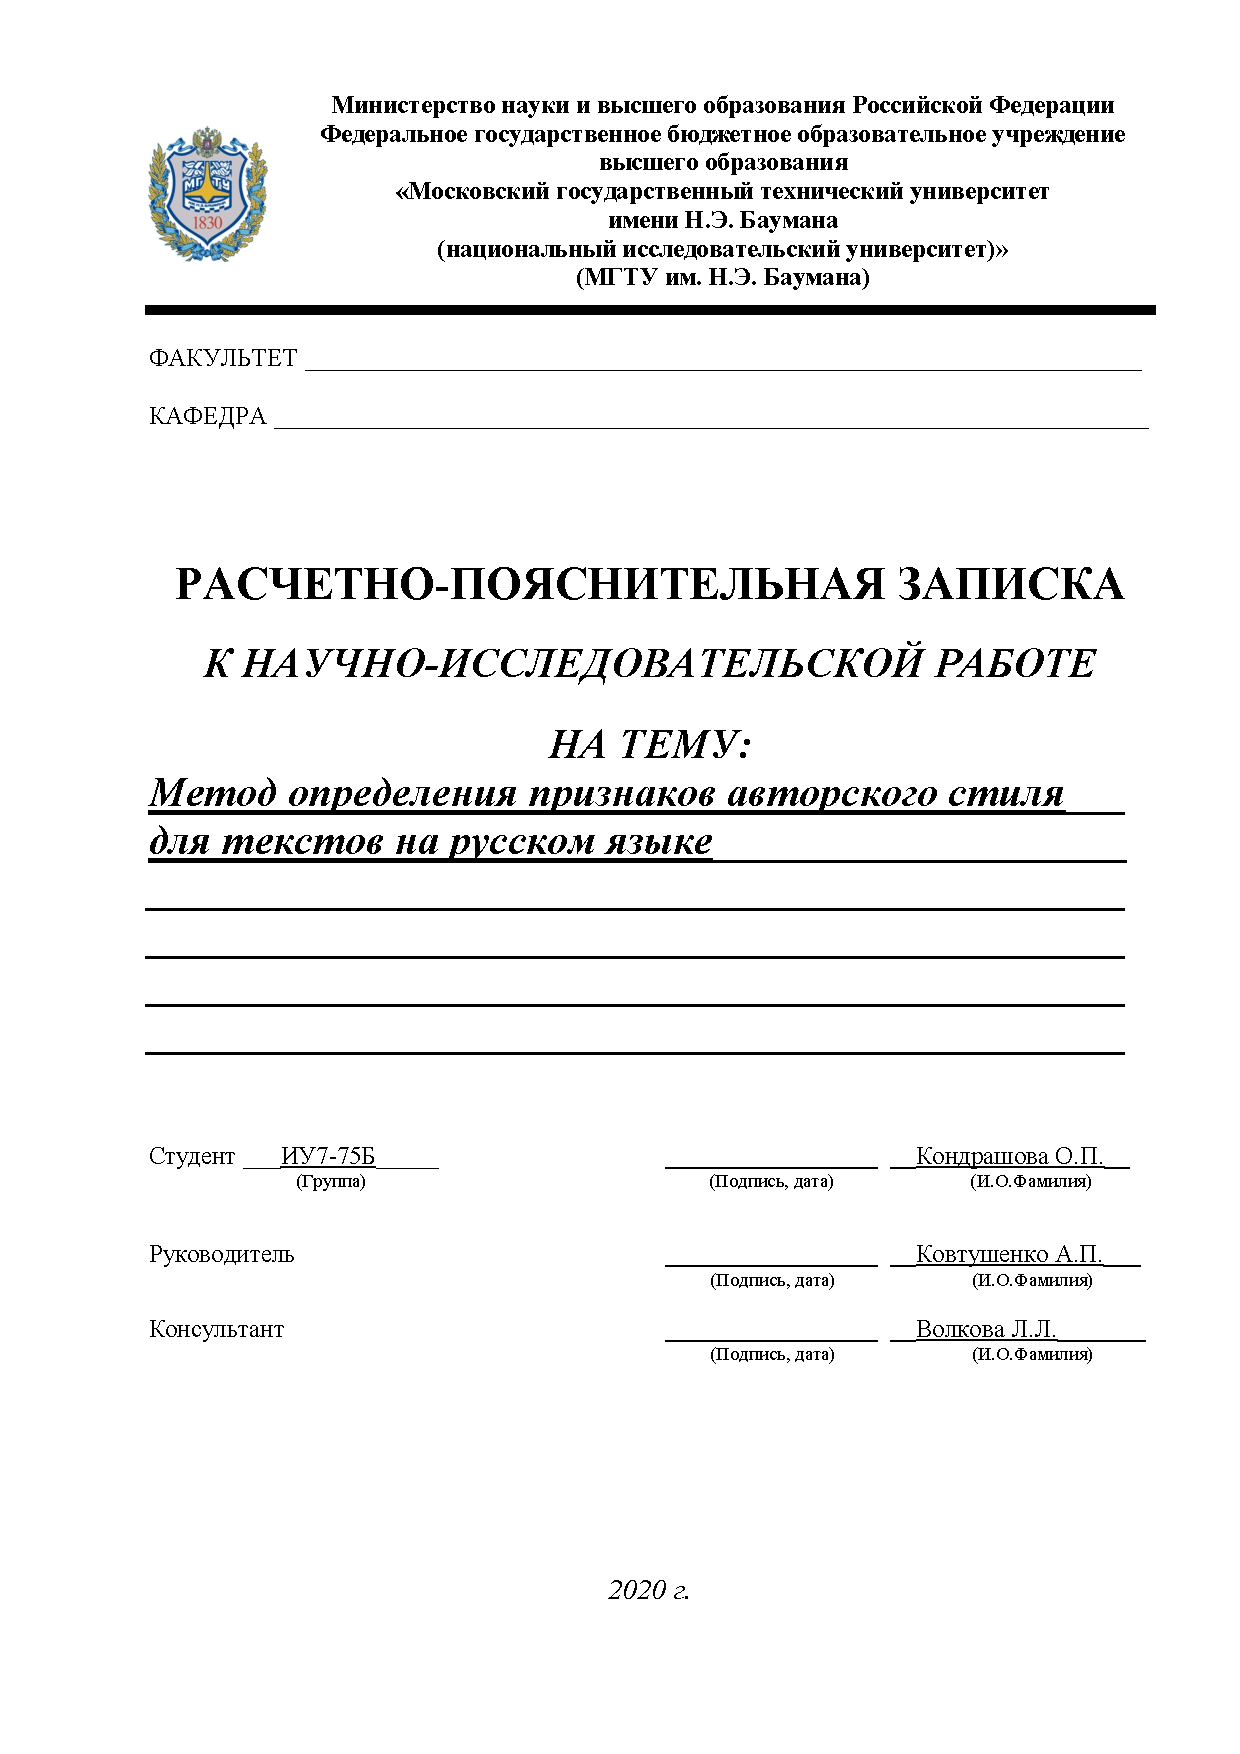
\includepdf[pages=-]{pages/title.pdf}
% пропущены страницы под тз и план (у меня их 2 тз и 1 план, итого 3, вам надо пропустить столько, сколько страниц у вас в тз и плане)


%\listoffigures                         % Список рисунков

%\listoftables                          % Список таблиц

%\NormRefs % Нормативные ссылки 
% Команды \breakingbeforechapters и \nonbreakingbeforechapters
% управляют разрывом страницы перед главами.
% По-умолчанию страница разрывается.

% \nobreakingbeforechapters
% \breakingbeforechapters

\tableofcontents

% \printnomenclature % Автоматический список сокращений

\Introduction
В последние годы очень быстрыми темпами развивается область  обработки естественных языков. Во  многом  это связано с тем, что с каждым годом объём текстовой информации, используемой человечеством,  увеличивается,  и  растёт  потребность  в  более  эффективных алгоритмах  обработки  и  анализа  документов,  написанных  на  естественных языках. Особо важную роль играет возможность определить автора текста, основываясь на его стилистических признаках.

Выявление признаков авторского стиля позволяет установить принадлежность текста определенному человеку. Актуальность данного направления в компьютерной лингвистике обусловлена необходимостью в выявлении плагиата или в создании рекомендательной системы для нахождения похожжих текстов. Для определения стиля автора необходимо выделить характерные признаки из принадлежащих ему текстов.


Целью данной работы является разработка метода определения признаков авторского стиля для текстов на русском языке.

Для достижения этой цели ставятся следующие задачи:

\begin{enumerate}
	\item изучить предметную область;
    \item проанализировать существующие решения;
    \item проанализировать алгоритмы классификации;
    \item разработать метод определения признаков авторского стиля;
    \item рспроектировать структуру ПО для проведения исследования;
    \item реализовать ПО;
    \item провести апробацию предложенного метода.
\end{enumerate}

Разрабатываемый метод позволит учитывать классификацию текстов на русском языке по авторскому стилю на основании результатов морфологического анализа, не задействуя более трудоемкий и менее доступный синтаксический анализ.


\mainmatter % это включает нумерацию глав и секций в документе ниже

\chapter{Аналитический раздел}
\label{cha:analytical}

В данном разделе рассматривается понятие авторского стиля и стилеметрических характеристик, исследуются алгоритмы классификации и существущие методы определения авторского стиля, анализируются их достоинства и недостатки. Также в этом разделе производится формализация решаемой задачи.

\section{Описание предметной области}

Под авторским стилем понимается совокупность характеристик, позволяющих установить авторство текста или выдвинуть предположение, кем может являться автор или к какой группе авторов он может принадлежать. К особенностям авторского стиля можно отнести грамматические конструкции, стилистические приемы, способы построения фраз и абзацев или любой другой набор признаков, который отличает конкретного автора от всех других. 

Раздел лингвистики, зани­мающийся измерением стилевых характеристик с целью систематиза­ции и упорядочения текстов, называется стилеметрией \cite{stylometry}. Объектом стилеметрии является текст, созданный конкретным ав­тором. Предметом ис­следования являются элементы стиля, которые понимаются как осо­бенности стиля конкретного автора. Стиль текста описывается как набор некоторых присущих ему  характеристик. В большинстве случаев в качестве характеризующих параметров текста выбираются статистические характеристики: количество использования определенных частей речи, знаков препинания, количество и длина предложений (измеренная в словах, слогах, знаках), объем словаря, количество полнозначных и служебных слов, средняя длина предложения в тексте и т.д.

Под авторским инвариантом понимаются стилеметрические характеристики, которые однозначно характеризует одного автора или небольшое число «близких авторов» \cite{invariant}. Анализируемые характеристики должны принимать существенно разные значения для произведений разных групп авторов. Для успешного установления авторства нужно, чтобы число «разных групп» было достаточно велико, и при этом каждая группа должна включать в себя небольшое количество близких по стилю произведений.

\section{Этапы обработки текстов на естественном языке}

В данном разделе будет выполнен обзор этапов обработки текстов на естественном языке.

\subsection{Токенизация}

Токенизация — этобазовый этап в автоматической обработке текстов, суть которого заключается в разбиении непрерывной строки на отдельные «слова» (токены) \cite{tokenization}. 

Текст на естественном языке состоит не только из букв, но и из символов: скобок, кавычек, тире. Если все символы, не являющиеся буквами или строками, заменить на пробелы, то слова, разделённые пробелами, можно объявить отдельными токенами. Однако возникает много нюансов, например, слово «каком-либо». При замене дефиса на пробел оказывается, что есть два слова: «каком» и «либо». На самом деле это одно слово, которое было бы правильнее не разделять.

На этапе токенизации также реашется задача разбиения текста на предложения. На этапе членения текста на предложения недостаточно только рассматривать точки перед большими буквами. Например, под данное правило не попадают инициалы. 

Токенизация состоит из нескольких этапов. В первую очередь текст приводится к нижнему регистру. На данном этапе можно потерять часть информации. Например, «ООО» может являться сокращением (общество с ограниченной ответственностью), а «ооо» — просто выражением эмоций.

Следующий этап — это замена всех знаков препинания и прочих символов на пробелы. Как было упомянуто выше, при наличии сложных составных слов (например, «красно-чёрный») заменять в них дефис на пробел не очень разумно: может потеряться смысл слова. 

Далее каждое слово, отделённое пробелом, объявляется отдельным токеном. На данном этапе стоит учитывать, что некоторые наборы слов должны рассматриваться как одно. Например, названия городов («Нижний Новгород»), или сокращения («к.т.н.», кандидат технических наук, это полезный термин при рассмотрении трёх букв вместе, но по отдельности они никакой информации не несут)  \cite{tutorial}. 

\subsection{Нормализация}

Следующий этап после токенизации — это нормализация слов в тексте, то есть приведение каждого слова к его начальной форме. 

Существует два основных подхода к нормализации: стемминг и лемматизация  \cite{tutorial}.

Стемминг - это подход, суть которого заключается в следующем: по некоторым правилам от каждого слова отрезается его окончание. Данный подход может работать некорректно в том случае, если при изменении формы слово меняется целиком (например, «был», «есть», «будет»).

Суть подхода лемматизации заключается в  использовании словаря, в который предварительно записано большое количество слов и их форм. В первую очередь слово проверяется по словарю. Если оно там есть, то по словарю можно найти, к какой форме можно привести данное слово. Иначе по определённому алгоритму выводится способ изменения данного слова, на основании него делаются выводы о начальной форме.

Лемматизация лучше подходит для работы с незнакомыми словами, но за счет поиска в словаре и алгоритма приведения к нормальной форме, является более медленным подходом по сравнению со стеммингом.


\section{Методы и решения определения авторского инварианта}

В данном разделе будут проанализированы существующие методы выделения признаков в тексте.

\subsection{Метод полного синтаксического анализа}

В области обработки текстов на естественном языке, как и в информатике в целом, под синтаксическим анализом понимается сопоставление лексем некоторого языка (естественного или формального) с его формальной грамматикой. Единицей синтаксического анализа текстов на естественном языке обычно является предложение.

С другой стороны, что более важно, в задаче понимания текста машиной синтаксический анализ – это построение такой структуры, которая позволяет приблизиться к некоторому эксплицитному формализованному представлению смысла текста. Но, в отличие от «глубокой» семантической структуры, которая строится в результате семантического анализа, синтаксическая структура обычно не связывает ЕЯ-конструкции с их значениями в некоторой предметной области. Синтаксическая структура может выступать либо как промежуточный результат, который является входом для семантического анализа, либо как удобное представление текста на ЕЯ для решения высокоуровневых прикладных задач.

Большинство моделей синтаксической структуры предложения  опираются либо на грамматику составляющих, предложенной в работах Ноама Хомского \cite{chomsky}, либо на грамматику зависимостей, для которой основополагающими считаются работы Люсьена Теньера \cite{tesniere} и Игоря Мельчука \cite{melcuk}.

На начальном этапе исследований в области компьютерной лингвистики большее внимание уделялось грамматике составляющих. Эта модель предполагает, что предложение ЕЯ может быть представлено в виде иерархии составляющих – проективных синтаксических групп, которые не могут частично пересекаться, но которые в свою очередь состоят из более мелких групп (быть вложенными), вплоть до атомарных групп – слов предложения. Такую иерархическую структуру называют деревом составляющих.

\subsection{Метод энтропийной классификации}

Метод классификации текстов, предложенный в работе \cite{entropy1} основывается на применении алгоритмов сжатия данных для задачи определения авторства. Также был сделан вывод о том, что простейший подход с использованием цепей Маркова первого порядка показывает хорошие результаты на файлах большого объема и плохие по сравнению с другими методами на отрывках длиной в 2 000–5 000 символов \cite{batura}. Предложенный метод был реализован в системе «Лингвоанализатор».

Существенным преимуществом метода энтропийной классификации является отсутствие необходимости в предварительной обработки текста. Суть данного метода заключается в том, чтобы добавлять текст, автор которого неизвестен, к текстам, характеризующим конкретного автора, и смотреть, насколько хорошо сжимается эта «добавка». Правильный исходный класс документа – это тот, на котором он сжимается лучше всего.

Проведенные автором эксперименты показывают, что подход с использованием цепей Маркова первого порядка позволяет получить точность 69\%  на файлах большого объёма (50-100 тысяч символов), но на небольших отрывках длиной в 2-5 тысяч символов проигрывает в точности другим методам. Наилучшие результаты показала программа rarw (точность 71\%), превзойдя точность других подходов в этой области.

\subsection{Система «Стилеанализатор»}

Проблему установления авторства текстов в \cite{analyzator} предлагается решать при помощи нейронных сетей и методов иерархической кластеризации. В качестве меры сравнения матриц частот появления признаков предлагается использовать меру Кульбака и меру $\chi$-квадрат. Под частотным признаком понимается любой признак стиля текста, допускающий возможность нахождения частоты его появления в тексте (например, число появления абзацев в тексте). На основе проведенных исследований разработан программный комплекс «Стилеанализатор».

Было предложено использовать нейронные сети, обучающиеся без учителя и предназначенные для обработки больших массивов многомерной информации, – самоорганизующиеся карты Кохонена (Self-organizing map – SOM). За последние годы это направление является одним из наиболее развивающихся. С помощью SOM-сетей решаются многие проблемы классификации, обработки естественного языка, изображений, тестирования и обучения \cite{batura}. Несмотря на широкое использование, SOM-сетям не хватает теоретической обоснованности: в основном они опираются на эмпирические результаты. В итоге был получен вывод о том, что в случае удачного нахождения универсального набора характеристик можно обрабатывать любое число авторов и текстов (большие массивы информации). Достаточно постоянно модифицировать карту, добавляя новые произведения, и оценивать, как они взаимодействуют с уже имеющимеся в базе.

Одним из серьезных недостатков метода является невозможность прогнозирования успешного результата. Генетический поиск на заданном наборе текстов может никогда не найти хороший вариант для разделения характеристик. Нет никакого критерия того, в правильном ли направлении движется поиск, верно ли он делает скачки, нужную ли скапливает информацию об исследуемом пространстве. 

Другой проблемой метода является его трудоемкость. Число загруженных текстов, которое напрямую влияет на качество поиска, требует больших ресурсов от вычислительной системы (большой объем памяти и мощный процессор). Для нахождения по-настоящему универсальных характеристик необходимо обработать не один десяток мегабайт текстов, чтобы можно было с уверенностью заявить об их универсальности.

\subsection{Система «Авторовед»}

Продолжение исследований по применению нейронных сетей в сочетании с методом опорных векторов при установлении авторства текстов нашло отражение в работе \cite{avtoroved}. Если задачу определения авторства сформулировать как задачу классификации, то одним из широко применяемых выходов является построение бинарного классификатора. Все тексты, включая обучающую часть выборки, разворачиваются в очень большой вектор, индексируемый словами. После этого имеются два множества точек из обучающей выборки в многомерном пространстве: принадлежащие данному автору и не принадлежащие ему. Для того чтобы разделить эти множества, нужно поделить пространство на две части. Самый простой способ сделать это – построить гиперплоскость. Такую гиперплоскость можно построить с помощью метода опорных векторов (SVM – Support Vector Machines). После этого для классификации текста с неизвестным автором достаточно проверить, в какую часть пространства он попал.

Помимо метода опорных векторов, в качестве инструментов для атрибуции текстов в работе \cite{avtoroved} были выбраны искусственные нейронные сети архитектуры многослойный перцептрон (MLP) и сети каскадной корреляции (CCN). CCN позволяют снизить временные затраты на обучение по сравнению с перцептроном за счет алгоритма автоматического построения топологии сети. SVM является наиболее точным из существующих сегодня методов классификации и в то же время наименее затратным по времени. Итоговое решение об авторе текста принимается ансамблем классификаторов по принципу мажоритарного голосования. В качестве характерных признаков текста для описания авторского стиля было предложено брать наиболее частые триграммы символов и наиболее частые слова русского языка.

Полученные методики были применены на практике для идентификации авторов коротких электронных сообщений во время внедрения программного комплекса, названного «Авторовед»,  в деятельность воинской части 51 952. Результаты показали, что авторство коротких текстов длиной 100 символов можно определить с точностью до 76±11 \% в случае двух потенциальных авторов. При решении частной задачи по определению автора сообщения интернет-форума была достигнута точность 89±8 %. Таким образом, предложенный метод дает довольно хорошие результаты на коротких электронных сообщениях, что выгодно отличает его от других ранее предложенных методов.

\subsection{Метод анализа длин слов}

Для поставленной задачи определения авторства текста существует также решение анализа стилистики текста, основанное на длине слов. Данное решение легло в основу программы «Худломер».

«Худломер» - это метод автоматической классификации функционального стиля текста на основе спектров длин слов. Программа позволяет определять следующие стили: разговорный стиль, стиль художественной литературы, газетно-информационный стиль, научно-деловой стиль. Автор Худломера - президент конкурса русской сетевой литературы ТЕНЕТА-РИНЕТ'2000, Леонид Делицин \cite{hoodlomer}.

\subsection{Метод выделения N-грамм}

Использование N-грамм характерно тем, что позволяетучитывать порядок слов. N-грамма — это последовательность из N идущих подряд слов в тексте.

N-грамма имеет в основе своего использования математическую модель и определяется следующим образом: «N-граммой на алфавите V называют произвольную цепочку длиной N, например последовательность из N букв алфавита V одного слова, одной фразы, одного текста или, в более интересном случае, последовательность из грамматически допустимых описаний N подряд стоящих слов» \cite{ngrams}.

Чем больше N, до которого будут найдены N-граммы, тем больше будет получено признаков. При этом увеличение параметра N может привести к переобучению. Например, если N — это длина текста, то у каждого документа будет уникальный признак, и алгоритм сможет переучиться под обучающую выборку.

N-граммы можно использовать не только на словах. В качестве токенов можно рассматривать отдельные символы в предложении. После нахождения таких токенов для них можно также вычислять N-граммы (буквенные N-граммы). Данный подход позволяет учитывать смайлы в тексте или известные слова в незнакомых формах. Часто буквенные N-граммы используют вместе с N-граммами по словам.

Skip-граммы — это чуть более расширенный подход к использованию N-грамм. Более точно они называются k-skip-n-граммы, это наборы из N токенов, причём расстояние между соседними должно составлять не более K токенов \cite{skipgrams}. Данный метод позволяет учитывать больше различных N-грамм в предложени, и в связи с этим, как правило, используется в языковом моделировании в сочетании с другими подходами. 

\section{Классификация текстов}

В данном разделе будут рассмотрены алгоритмы классификации текстов.

\subsection{Алгоритм наивной  байесовской классификации}

Наивный байесовский классификатор — простой вероятностный классификатор, основанный на применении теоремы Байеса со строгими (наивными) предположениями о независимости. Целью классификации является поиск наилучшего класса для документа.

В зависимости от точной природы вероятностной модели, наивные байесовские классификаторы могут обучаться очень эффективно. Во многих практических приложениях для оценки параметров для наивных байесовых моделей используют метод максимального правдоподобия; другими словами, можно работать с наивной байесовской моделью, не веря в байесовскую вероятность и не используя байесовские методы.

Достоинством наивного байесовского классификатора является малое количество данных, необходимых для обучения, оценки параметров и классификации [1].

\subsection{Алгоритм опорных векторов}

Метод опорных векторов — набор схожих алгоритмов обучения с учителем, использующихся для задач классификации и регрессионного анализа. Принадлежит семейству линейных классификаторов и может также рассматриваться как специальный случай регуляризации по Тихонову. Особым свойством метода опорных векторов является непрерывное уменьшение эмпирической ошибки классификации и увеличение зазора, поэтому метод также известен как метод классификатора с максимальным зазором.

Основная идея метода — перевод исходных векторов в пространство более высокой размерности и поиск разделяющей гиперплоскости с максимальным зазором в этом пространстве. Две параллельных гиперплоскости строятся по обеим сторонам гиперплоскости, разделяющей классы. Разделяющей гиперплоскостью будет гиперплоскость, максимизирующая расстояние до двух параллельных гиперплоскостей. Алгоритм работает в предположении, что чем больше разница или расстояние между этими параллельными гиперплоскостями, тем меньше будет средняя ошибка классификатора [1].

\subsection{Случайный лес}

Алгоритм случайного леса применяется для задач классификации, регрессии и кластеризации. Основная идея заключается в использовании большого ансамбля решающих деревьев, каждое из которых само по себе даёт очень невысокое качество классификации, но за счёт их большого количества результат получается более точным.

Случайные леса могут быть естественным образом использованы для оценки важности переменных в задачах регрессии и классификации.  В задаче регрессии ответы решающих деревьев усредняются, в задаче классификации принимается решение голосованием по большинству. 

Все деревья строятся независимо по следующей схеме.
\begin{enumerate}
\item выбирается подвыборка обучающей выборки заданного размера – по ней строится дерево (для каждого дерева — своя подвыборка);
\item для построения каждого расщепления в дереве ппроссматриваются случайных признаков (для каждого нового расщепления — свои случайные признаки).
\item выбирается наилучший признак и расщепление по нему (по заранее заданному критерию). Дерево строится, как правило, до исчерпания выборки (пока в листьях не останутся представители только одного класса), но в современных реализациях есть параметры, которые ограничивают высоту дерева, число объектов в листьях и число объектов в подвыборке, при котором проводится расщепление [4].
\end{enumerate}

\section{Последовательность решения задачи}

Основываясь на проведённом анализе предметной области, цель данной работы можно уточнить следующим образом. 

Необходимо разработать метод определения признаков авторского стиля для текстов на русском языке. 
Первым этапом предлагаемого метода является классификация текстов из обучающей выборки, у которых заранее известен автор. Для каждого из текстов из обучающей выборки провести N-граммный разбор предложений и провести подсчет статистического распределения N-грамм, характерных для стиля каждого автора. Сами N-граммы будут представлять собой связку из частей речи, то есть кортеж из словоформ будет представлен как кортеж из частей речи этих словоформ (например, существительное-глагол-прилагательное-существительное).  
После анализа каждого текста из имеющейся базы будет получен набор данных – статистическая характеристика распределения N-грамм с определенными частями речи, характерная для конкретного автора. Для оценки важности выделенной N-граммы для текста заданного автора предлагается использовать статистическую меру TF-IDF.

Следующий этап метода – проведение морфологического и N-граммного анализа для нового текста, не входящего в обучающую выборку. Завершается метод классификацией текста на основе полученного распределения частеречных N-грамм. В результате можно установить автора текста или выдвинуть предположение, кто может быть автором (в таком случае принятие решения предоставляется эксперту).

После определения авторства текста, его можно будет сохранить в имеющуюся базу и отнести к определенному авторскому стилю результаты анализа. Таким образом, метод подразумевает дообучение по мере добавления и анализа новых текстов.

Также необходимо разработать программное обеспечение (ПО), использующее разработанный метод, провести параметризацию метода и исследование качества работы разработанного метода.


\section{Выводы}

В данном разделе были рассмотрены этапы обработки текстов на естественном языке, методы выделения признаков в тексте. Были проанализированы алгоритмы классификации текстов. В ходе проведенного анализа было установлено, что для текстовых данных, как правило, используют линейные алгоритмы, т.к. они масштабируемы, могут работать с большим количеством признаков, на очень больших выборках. В качестве алгоритма классификации был выбран наивный Байес.
\chapter{Конструкторский раздел}
\label{cha:design}

В данном разделе рассматривается проектирование структуры программного обеспечения и требования к нему.

\section{Функциональная модель предлагаемого метода}

На рис. \ref{fig:idef0} представлена функциональная схема предлагаемого метода 
определения признаков авторского стиля в нотации IDEF0, нулевой уровень.

\begin{figure}[H]
    \centering
    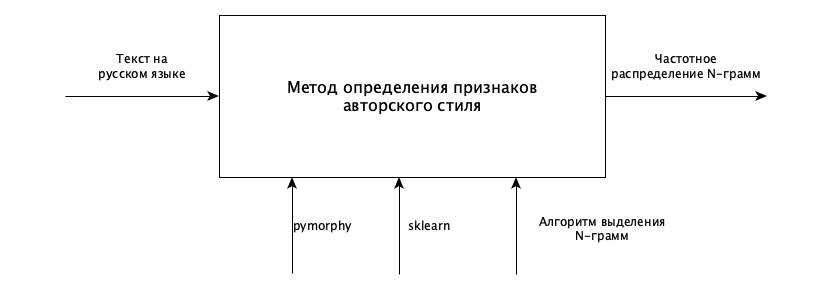
\includegraphics[scale=0.5]{img/idef0.png}
    \caption{Функциональная схема метода определения признаков авторского стиля}
    \label{fig:idef0}
\end{figure}

\section{Требования к программному обеспечению}

Необходимо разработать программное обеспечение, которое получает на вход текст на русском языке, и с помощью метода выделения N-грамм определяет признаки текста: морфологические параметры N-грамм, мера TF\_IDF. На выходе получаем частотное распределение N-грамм с определенными частями речи.

\section{Выводы}

В данном разделе был рассмотрен процесс проектирования структуры программного обеспечения и требования, выдвигаемые  к программному обеспечению.

%\include{50-research}

\backmatter %% Здесь заканчивается нумерованная часть документа и начинаются ссылки и
            
\Conclusion % заключение к отчёту

В ходе данной научно-исследовательской работы были выполнены следующие задачи:

\begin{enumerate}
	\item изучены этапы обработки текстов на естественном языке;
    \item произведен анализ существующих методов выделения признаков в тексте;
    \item проанализированы алгоритмы классификации;
    \item разработана функциональная модель и требования к программному обеспечению.
\end{enumerate}%% заключение

\begin{thebibliography}{}
\bibitem{stylometry} Мартыненко Г. Я. (2015). Стилеметрия: Возникновение и становление в контексте междисциплинарного взаимодействия. Часть 2. Первая половина XX в.: Расширение междисциплинарных контактов стилеметрии. СТРУКТУРНАЯ И ПРИКЛАДНАЯ ЛИНГВИСТИКА, (11), 9-28.
\bibitem{invariant} Фоменко В.П., Фоменко Т.Г. Авторский инвариант русских литературных текстов. Предисловие А.Т. Фоменко // Фоменко А.Т. Новая хронология Греции: Античность в средневековье. Т. 2. М.: Изд-во МГУ, 1996. С.7 68-820.
\bibitem{tokenization} Ермакович М.В. Автоматическое определение границ слова в русском тексте с помощью комплекса лингвистических правил. Компьютерная лингвистика и интеллектуальные технологии: по материалам международной конференции «Диалог 2017» Москва, 31 мая — 3 июня 2017.
\bibitem{tutorial} Автоматическая обработка текстов на естественном языке и компьютерная лингвистика: учеб. пособие / Большакова Е.И., Клышинский Э.С., Ландэ Д.В., Носков А.А., Пескова О.В., Ягунова Е.В.
\bibitem{synt} Шелманов А.О., Исследование методов автоматического анализа текстов и разработка интегрированной системы семантико-синтаксического анализа.
\bibitem{chomsky} Chomsky N. Three models for the description of language // IRE Transactions on Information Theory. — 1956. — Vol. 2, no. 3. — P. 113–124.
\bibitem{tesniere} Tesnière L. Elements de syntaxe structurale. — Editions Klincksieck, 1959.
\bibitem{melcuk} Mel’cuk I. A. Dependency syntax: theory and practice. — ŠUNY Press, 1988. — P. 428.
\bibitem{entropy1} Хмелев Д.В. Классификация и разметка текстов с использованием методов сжатия данных [электронный ресурс] - режим доступа: URL: http://compres­sion.ru/download/articles/classif/intro.html (дата обращения: 14.03.2021).
\bibitem{batura} Батура Т. В. Формальные методы установления авторства текстов и их реализация в программных продуктах // Программные продукты и системы. 2013. №4. 
\bibitem{analyzator} Шевелев О. Г. Методы автоматической классификации текстов на естественном языке : учебное пособие / О. Г. Шевелев ; науч. ред. В. В. Поддубный ; Том. гос. ун-т. - Томск : ТМЛ-Пресс, 2007. 
\bibitem{avtoroved} Романов А.С., Мещеряков Р.В. Компьютерная лингвистика и интеллектуальные технологии: По материалам ежегодной Международной конференции «Диалог»(Бекасово, 26-30 мая 2010 г.). М.: Изд-во РГГУ
\bibitem{hoodlomer} Программы анализа и лингвистической обработки текстов. Русская виртуальная библиотека [электронный ресурс] - режим доступа: URL: https://rvb.ru/soft/catalogue/c01.html (дата обращения: 20.12.2020).
\bibitem{ngrams} Гудков В. Ю., Гудкова Е. Ф. N-граммы в лингвистике // Вестник Челябинского государственного университета. 2011. № 24 (239). Филология. Искусствоведение. Вып. 57. С. 69–71.
\bibitem{skipgrams} Guthrie David, Allison Ben, Liu Wei, Guthrie Louise, Wilks Yorick. (2006). A Closer Look at Skip-gram Modelling. Proc. of the Fifth International Conference on Language Resources and Evaluation. 
\end{thebibliography}

\end{document}

%%% Local Variables:
%%% mode: latex
%%% TeX-master: t
%%% End:
